\documentclass[11pt]{article}
\usepackage[margin=0.9in]{geometry}
\usepackage{amsmath,amssymb,booktabs,graphicx,hyperref,xcolor,caption}
\hypersetup{colorlinks=true,linkcolor=blue!50!black,urlcolor=blue!50!black,citecolor=blue!50!black}
\setlength{\parskip}{0.45em}\setlength{\parindent}{0pt}
\captionsetup{font=small,labelfont=bf}
\graphicspath{{../figures/}}
\newcommand{\ED}[1]{{\color{red}[ED: #1]}}
\newcommand{\nuh}{\nu=1/2}
\newcommand{\nut}{\nu\approx0.3}
\newcommand{\nutw}{\nu\approx0.2}
\title{Reference answer: a layered oxide built from perovskite-type blocks\\[0.3em]
\large Effective theory, phase diagram, interpretation of the data, ARPES prediction and Luttinger surface}
\author{Prepared with the measurement data in \texttt{measurements.json}; all energies in units of $D$}
\date{29 October 2026}
\begin{document}
\maketitle

\section*{Summary of the answer}

\textbf{Effective theory.} One orbital per transition-metal site on a \emph{bilayer} square lattice (two metal--oxygen planes per perovskite block, sites $(i,\ell)$, $\ell=1,2$), with in-plane nearest- and next-nearest-neighbour hopping in each layer and an antiferromagnetic exchange on every inter-layer bond (``rung''):
\begin{equation}
H=-t_1\!\!\sum_{\langle ij\rangle,\ell,\sigma}\!\!\big(c^\dagger_{i\ell\sigma}c_{j\ell\sigma}+\text{h.c.}\big)
 -t_2\!\!\sum_{\langle\!\langle ij\rangle\!\rangle,\ell,\sigma}\!\!\big(c^\dagger_{i\ell\sigma}c_{j\ell\sigma}+\text{h.c.}\big)
 +J\sum_i \mathbf S_{i1}\!\cdot\!\mathbf S_{i2}-\mu\sum_{i\ell\sigma}n_{i\ell\sigma},
\label{eq:H}
\end{equation}
with $t_1=1.02\pm0.03$, $t_2=0.20\pm0.01$, $J=8.0\pm0.4$ (all in units of $D$). Inter-layer single-particle hopping and an on-site Hubbard term are not needed: the data bound them to $|t_\perp|\lesssim0.15$ and $|U|\lesssim0.5$. The filling $\nu$ is the fraction of the Brillouin zone filled per spin and per layer.

\textbf{Phases.} At $\nuh$ (one electron per site) the ground state is a featureless, fully symmetric insulator built from inter-layer spin singlets on every rung (a ``symmetric mass generation'' insulator, equivalently a Mott insulator of rung pairs). It has a single-particle gap $8.04$ and a spin (triplon) gap $5.5$ and breaks no symmetry, which is what the unchanged diffraction and the single NMR line require. Doping in either direction produces an inter-layer spin-singlet superconductor with an $s$-wave (on-rung) gap. Near $\nuh$ the pairs are tightly bound rung singlets and $T_c$ is limited by phase stiffness, which vanishes at the pair-Mott point $\nuh$; at lower density the state is BCS-like. The $\nut$ crystal is superconducting below $T_c=0.36$, is a paired but phase-incoherent liquid with a pseudogap (a single-particle gap that fills but does not close) up to $T\approx4$, and is an incoherent metal above. The $\nutw$ crystal is a superconductor with sharp Bogoliubov quasiparticles below $T_c=0.59$ ($2\Delta/T_c=5.9$; Hebel--Slichter peak at $T=0.47$) and a Fermi-liquid metal above.

\textbf{Predictions.} At $\nuh$ ARPES shows no Fermi surface; the occupied band is a copy of the bare band with \emph{half} its width at leading order (hole motion through a singlet background costs a factor $1/2$; the exact cluster spectra give $0.33$--$0.39$), its top at $(1/2,1/2)$ at $-4$ and its bottom at $(0,0)$; its spectral weight is largest near $(0,0)$ and smallest near $(1/2,1/2)$. The Green's function recovered from this spectrum, with $\omega=0$ at the gap midpoint, has a closed surface of zeros. In the leading strong-coupling theory it is the contour $\varepsilon(k)=-4t_2$, which encloses $0.31$ of the zone around $(0,0)$; with the exact cluster Green's function (3$\times$3 bilayer torus) the zeros form a band inside the gap that disperses by only $1.2$ and crosses the midpoint on the contour $\varepsilon(k)\approx1.9$, so that the zero surface encloses $0.74$--$0.81$ of the zone around $(0,0)$. Neither value is $\nu=0.50$: the Luttinger count applied to zeros fails in this insulator, and the fraction is not even robust (moving the reference energy by $\pm0.3$ inside the $8.6$ gap moves it between $0.46$ and $0.91$), because the zero surface is fixed by the momentum dependence of the residues and of the incoherent weight rather than by a conserved quantity. At $\nutw$ ARPES shows Bogoliubov bands with sharp back-bending on a small locus around $(0,0)$ (the contour $\varepsilon(k)=\mu=-2.46$, enclosing $0.16$ of the zone, inside the normal-state Fermi surface because pairing has pulled $\mu$ down) and gap $1.73$. At $\nut$ the gap is larger ($2.5$), the back-bending is smeared, the coherence peaks are absent and the weight is asymmetric between removal and addition.

\section{Reading the data}

\subsection{Structure and counting}
The in-plane period is the metal--metal distance at all temperatures, the transition-metal sites stay equivalent, and no peak appears or splits on cooling: the low-temperature states break neither translation, nor the fourfold rotation, nor any symmetry that would make the metal sites inequivalent. A ``layered oxide built from perovskite-type blocks'' is a Ruddlesden--Popper-type stack; the smallest block that carries one band ``dominated by a single orbital with some admixture'' and that can be gapped at $\nuh$ without breaking a symmetry is a \emph{bilayer}. The counting argument is the Lieb--Schultz--Mattis constraint: with one electron per site, a single-layer square lattice cannot be a symmetric gapped insulator (odd number of electrons per unit cell), whereas a bilayer has two electrons per in-plane unit cell and can. The $\nuh$ data (hard gap, no new diffraction peaks, single NMR line, activated spin relaxation with a gap different from the charge gap) are exactly this situation. The two sites of a rung are related by the mirror that exchanges the layers, so they are crystallographically equivalent, as stated.

\subsection{Quantities extracted from the curves}
All fits are least-squares fits of the full traces (Fig.~\ref{fig:fits}); the uncertainties quoted below are the spread between independent determinations plus the sensitivity to the broadening model, which exceed the statistical errors.

\begin{figure}[h]\centering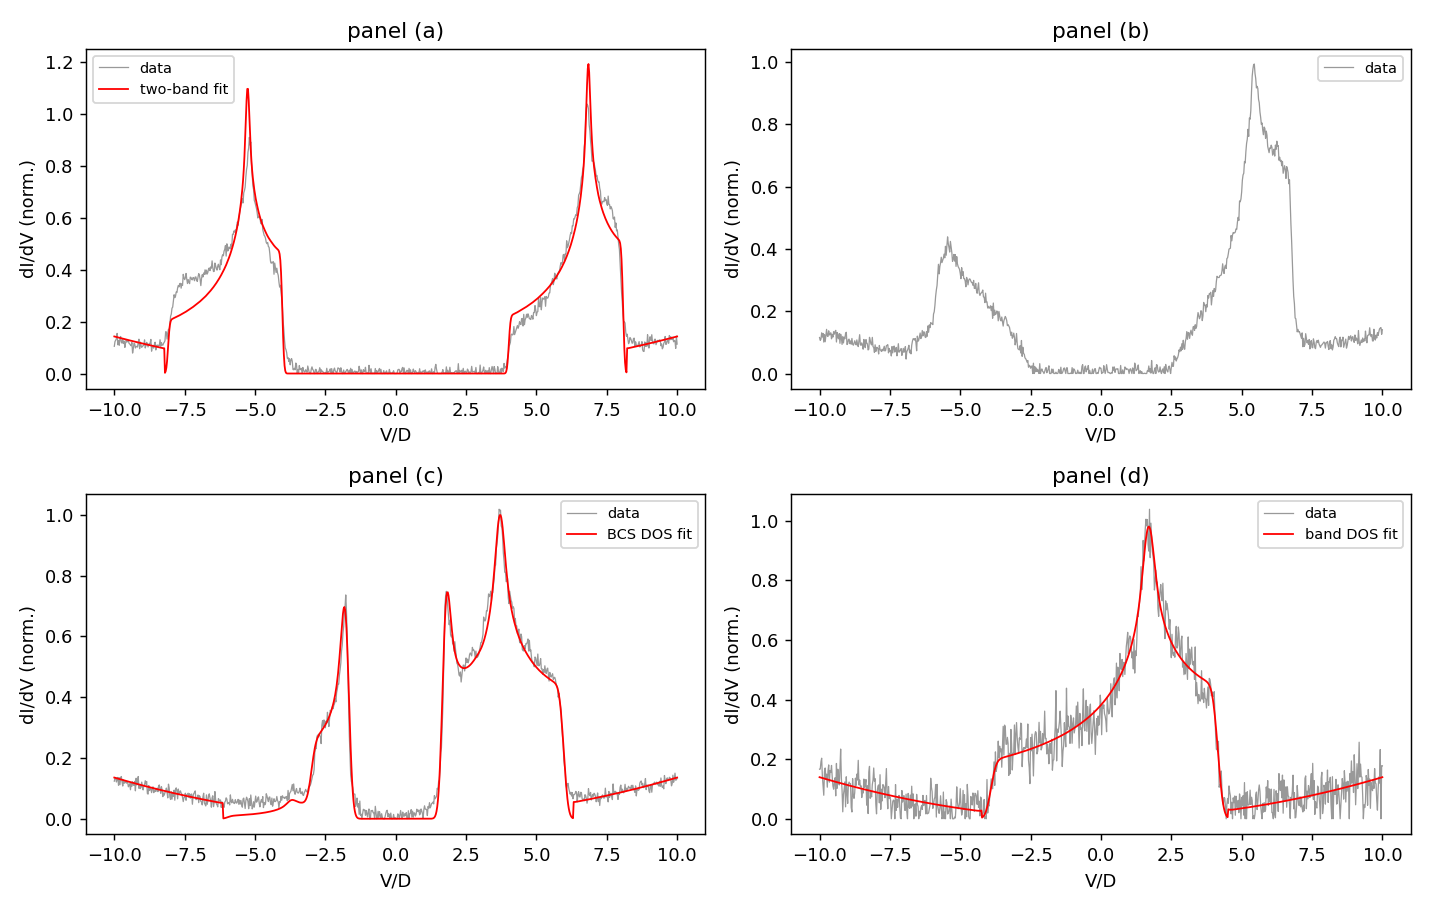
\includegraphics[width=0.95\textwidth]{fit_sts.png}
\caption{STS traces (grey) and fits (red). (a) two-band strong-coupling density of states (DOS) with $t_1,t_2$ and the two band offsets free; (c) BCS DOS of the $t_1$-$t_2$ band with $\mu$ and $\Delta$ free; (d) bare-band DOS with $t_1,t_2,\mu$ free. Panel (b) is analysed model-free. A $V^2$ background of $0.11$ at $|V|=9$ (other bands) is included outside the gaps.}
\label{fig:fits}\end{figure}

\begin{table}[h]\centering\footnotesize
\begin{tabular}{p{2.5cm}p{4.3cm}p{4.8cm}p{3.4cm}}\toprule
curve & quantity & value & how \\ \midrule
STS (d), $\nut$, high $T$ & bandwidth $8t_1$; van Hove at $4t_2-\mu$ & $t_1=1.009$, $t_2=0.197$, $\mu_N=-0.91$ & bare-band DOS fit; $\nu(\mu_N)=0.301$ \\
STS (a), $\nuh$ & gap edges; side-band width $4t_1$; van Hove $2t_2$ above each side-band centre & edges $\pm4.02$, $\Delta_c=8.04$; $t_1=1.016$, $t_2=0.198$ & two-band fit, particle/hole weight ratio $1.08$ \\
STS (c), $\nutw$ & BCS coherence peaks; van Hove at $\sqrt{(4t_2-\mu)^2+\Delta^2}$ & $\Delta=1.73$, $\mu=-2.46$ (occupied fraction $0.20$), $t_1=1.020$, $t_2=0.205$ & BCS DOS fit \\
STS (b), $\nut$, low $T$ & full gap, no coherence peak & edges $-2.48/+2.50$; peaks $-5.4/+5.45$ (heights $0.41/0.95$); outer edges $-5.9/+6.9$ & thresholds \\
NMR $\nuh$ & $1/(T_1T)\propto e^{-\Delta_s/T}$ & $\Delta_s=5.5\pm0.2$ & weighted Arrhenius fit, $T\le2$ \\
NMR $\nut$ & activated, no peak, two slopes; Korringa for $T\ge4$ & $2.47\pm0.09$ below $T_c$; $1.03\pm0.10$ for $0.4<T<2$ & same \\
NMR $\nutw$ & Hebel--Slichter peak $2.27\times$ Korringa at $T=0.47$, then $e^{-\Delta/T}$; Korringa above & slope $1.74\pm0.06$ below the peak & same \\
resistivity $\nuh$ & activated & $E_a=3.72\pm0.05$ & $\ln\rho$ vs $1/T$ \\
resistivity $\nut$ & zero below $T_c$; rises on cooling above & $T_c=0.36\pm0.04$, slope $0.90\pm0.04$ & onset of finite $\rho$ \\
resistivity $\nutw$ & zero below $T_c$; metallic above & $T_c=0.59\pm0.04$ & onset \\ \bottomrule
\end{tabular}
\caption{Numbers extracted from the measurement data (units of $D$).}\label{tab:data}\end{table}

Three independent facts fix the hoppings. The high-temperature trace (d) is a single two-dimensional tight-binding band of width $8t_1$ with one logarithmic van Hove peak; its position relative to the band edges ($5.6$ above the lower edge, $2.4$ below the upper one) gives $t_2/t_1=0.20$ and its sign ($t_2>0$ in the convention of Eq.~\ref{eq:H}, van Hove above the band centre). The absence of a second van Hove peak bounds an inter-layer hopping: a bonding--antibonding splitting $2t_\perp$ larger than the peak width ($\approx0.3$) would be visible, so $|t_\perp|\lesssim0.15$. The free-band filling of the fitted $\mu_N$ is $0.301$, i.e.\ the ``$\nu\approx0.3$'' crystal is at $\nu=0.30$; the same band with the BCS fit of (c) gives an occupied fraction $\sum_kv_k^2=0.20$ for the other crystal, with a paired chemical potential $\mu=-2.46$ that lies $0.54$ below the normal-state value of the same density ($-1.92$). In the half-filled trace (a) each side band is $4t_1$ wide with its van Hove peak $2t_1-4t_2=1.2$ below the hole-side edge and $2t_1+4t_2=2.8$ above the particle-side edge: both side bands are the bare band with \emph{half} the width, the fingerprint of a hole or an electron moving through a background of rung singlets (Sec.~\ref{sec:theory}).

\section{Task 1: the effective theory}\label{sec:theory}

\textbf{Degrees of freedom, lattice, unit cell.} Spin-1/2 fermions $c_{i\ell\sigma}$ in one Wannier orbital per transition-metal site, on a bilayer square lattice: $i$ labels the sites of a square lattice with the measured metal--metal distance, $\ell=1,2$ the two planes of the block. The unit cell is one rung (two sites); it is the crystallographic cell, since no symmetry is broken. $\nu=1$ is four electrons per rung, $\nuh$ is two, i.e.\ one electron per site.

\textbf{Hamiltonian.} Eq.~\eqref{eq:H}: $t_1$ nearest-neighbour and $t_2$ next-nearest-neighbour in-plane hopping (identical in both layers), an antiferromagnetic Heisenberg exchange $J>0$ across every rung, and the chemical potential. Two further terms could be present and are bounded rather than needed: an inter-layer hopping $t_\perp\sum c^\dagger_{i1\sigma}c_{i2\sigma}+\text{h.c.}$, $|t_\perp|\lesssim0.15$ (one van Hove peak in (d)), and an on-site repulsion $U\sum n_{i\ell\uparrow}n_{i\ell\downarrow}$, $|U|\lesssim0.5$ (it would raise the charge gap by $\approx U$ without raising the spin gap, Sec.~\ref{sec:J}). Physically, $J$ is the super-exchange generated by the inter-layer hopping and the Hund/Hubbard interactions of the parent orbital; in the effective theory it is kept as an independent coupling and $t_\perp$ is dropped because the bilayer band in (d) shows no splitting.

\textbf{Symmetries the model has.} Charge U(1); spin SU(2) (rotations acting on both layers together); the space group of the square bilayer (translations, $C_{4v}$ in the plane, and the mirror $\ell\leftrightarrow\bar\ell$ that exchanges the layers); time reversal. Because no term moves an electron between the layers, the model also has an \emph{emergent} U(1)$\times$U(1): the particle number of each layer is separately conserved. \textbf{Symmetries it lacks.} Particle--hole symmetry (broken by $t_2$; it would be restored for $t_2=0$ on the bipartite lattice); independent spin rotations of the two layers (broken by $J$ to the diagonal SU(2)); and, in the real crystal, the layer U(1)$\times$U(1) is only approximate ($t_\perp\ne0$). The low-temperature states discussed below preserve every symmetry of the crystal; the superconductor breaks only the charge U(1).

\textbf{Coefficients.} Table~\ref{tab:coef}. $t_1$ and $t_2$ follow from the three STS traces (previous section). $J$ follows from the half-filled charge gap: to leading order in $t/J$ the gap is $\Delta_c=\tfrac32J-4t_1$ (Sec.~\ref{sec:sc}), giving $J=\tfrac23(\Delta_c+4t_1)=8.07$; exact diagonalization at $J=8$ reproduces both the charge gap and the spin gap within their uncertainties (Sec.~\ref{sec:J}), and the sensitivities $\partial\Delta_c/\partial J$ and $\partial\Delta_s/\partial J$ (Sec.~\ref{sec:J}) convert the gap uncertainties and the finite-size spread into $\pm0.4$ on $J$.

\begin{table}[h]\centering\footnotesize
\begin{tabular}{p{1.7cm}p{5.0cm}p{2.0cm}p{6.1cm}}\toprule
coefficient & value & uncertainty & determined from \\ \midrule
$t_1$ & $1.02\,D$ & $\pm0.03$ & band width in (d); side-band widths in (a); BCS fit of (c) \\
$t_2$ & $0.20\,D$ & $\pm0.01$ & van Hove position in (d); van Hove--edge distances in (a) and (c) \\
$J$ & $8.0\,D$ & $\pm0.4$ & charge gap $8.04$ in (a) with the strong-coupling relation checked by ED; spin gap $5.5$ from NMR \\
$t_\perp$ & $0$ & $|t_\perp|<0.15$ & single van Hove peak in (d) \\
$U$ & $0$ & $|U|<0.5$ & charge gap and spin gap together \\
$\mu$ & $\nuh$: gap midpoint; $\nut$: $-0.91$ (normal state); $\nutw$: $-2.46$ (paired; normal state $-1.92$) & $\pm0.03$ & fits of (d) and (c), relative to the band centre \\ \bottomrule
\end{tabular}
\caption{Coefficients of Eq.~\eqref{eq:H} (units of $D$).}\label{tab:coef}\end{table}

\subsection{Why this is the most credible theory}
A hard, momentum-independent gap at one electron per site can come from a band insulator, from magnetic order, from an exciton (inter-layer particle--hole) condensate, or from an interaction-generated symmetric gap. A band insulator needs two bands per cell and would show a bonding--antibonding structure in (d); it does not. Magnetic order would split the NMR line or add a hyperfine field, and together with the nesting of the half-filled band it would fold the zone; neither happens. An exciton condensate with the nesting vector $(1/2,1/2)$ doubles the unit cell and adds superlattice peaks; the diffraction excludes it, and a uniform inter-layer exciton condensate would make the two layers inequivalent (it breaks the layer mirror), which contradicts the equivalence of the sites. What remains is a symmetric gapped state, which is possible precisely because the cell holds two electrons. The simplest interaction that produces it is an inter-layer singlet coupling $J$: for $J\gg t$ every rung forms a spin singlet, all symmetries are kept, and the spectrum has exactly the structure seen in (a), in the NMR and in the resistivity (Sec.~\ref{sec:data}). The same coupling is attractive for an inter-layer singlet pair, so it produces the superconductivity of the doped crystals with an isotropic (on-rung, $s$-wave) gap, again without breaking a lattice symmetry.

\subsection{Strong-coupling structure at $\nuh$}\label{sec:sc}
At $t=0$ each rung with two electrons is a singlet at energy $-\tfrac34J$; a rung with one or three electrons has energy $0$. Removing an electron from the singlet product state creates a ``holon'' (one electron on the rung) and adding one creates a ``trion'' (three electrons); each costs $\tfrac34J$. To first order in $t$, a holon or trion of layer $\ell$ and spin $\sigma$ hops within layer $\bar\ell$ with amplitude $t_{ij}/2$ (the two singlet overlaps give $1/\sqrt2\cdot1/\sqrt2$), so both carry the dispersion $\varepsilon(k)/2$ with $\varepsilon(k)=-2t_1(\cos k_x+\cos k_y)-4t_2\cos k_x\cos k_y$, and the Green's function is
\begin{equation}
G(k,\omega)=\frac{Z_h(k)}{\omega-E_h(k)}+\frac{Z_p(k)}{\omega-E_p(k)},\qquad E_{p,h}(k)=\pm\tfrac34J+\tfrac12\varepsilon(k)\;(+\text{const}),\qquad Z_h(k)=n(k),
\label{eq:G}
\end{equation}
with $Z_h=Z_p=\tfrac12$ at this order. The charge gap is $\Delta_c=\tfrac32J-\tfrac12(\varepsilon_{\max}-\varepsilon_{\min})=\tfrac32J-4t_1$ (hole edge at $(1/2,1/2)$, particle edge at $(0,0)$). A rung triplet (``triplon'') costs $J$; to second order it hops with amplitude $4t^2/J$ and its band minimum is at $(1/2,1/2)$. Removing a whole singlet pair leaves an empty rung that hops with $t_b=8t^2/3J=0.33$ and repels another empty rung on a neighbouring site with $V=4t^2/J=0.5$ (two-rung second-order theory, \texttt{code/strong\_coupling.py}); the doped holes are therefore hard-core bosons of charge $2e$, which is the origin of the superconductivity near $\nuh$ and of the vanishing of its $T_c$ at the pair-Mott point $\nuh$.

\subsection{Exact-diagonalization check of the gaps and of $J$}\label{sec:J}
Table~\ref{tab:gaps} compares the two gaps of the half-filled model at $t_1=1$, $t_2=0.2$, $J=8$ from the leading-order theory, from second-order perturbation theory and from exact diagonalization of two bilayer tori (Sec.~8) with the measured values. The charge gap is the sum of the lowest electron-addition energy at $(0,0)$ and the lowest removal energy at $(1/2,1/2)$ (periodic and antiperiodic boundary conditions, respectively, on the $3\times3$ torus); the spin gap is the lowest rung-odd triplet excitation at $(1/2,1/2)$ (the $3\times3$ torus does not contain this momentum; its value is the three-harmonic extrapolation of the triplon poles at $(0,0)$, $(1/3,0)$ and $(1/3,1/3)$, which are $8.47$, $7.36$, $6.33$). Second-order perturbation theory undershoots the spin gap because the virtual states it sums over (a holon--trion pair at $3J/2$ or $J/2$ above the initial state) are not far from the two bands they belong to; exact diagonalization settles both gaps. Within the exact relations the measured gaps correspond to $J=7.6$ (charge gap) and $J=8.0$ (spin gap), and within the leading-order relation to $J=8.1$; the spread between the two tori ($0.6$ in $\Delta_c$, $0.2$ in $\Delta_s$) is the finite-size uncertainty. The sensitivities, from the $4\times2$ torus at $J=7$, $8$ and $9$, are $\partial\Delta_c/\partial J=1.45$ and $\partial\Delta_s/\partial J=1.03$ (leading order $1.5$ and $1$). We quote $J=8.0\pm0.4$ and use $J=8$ throughout. An on-site $U$ enters both gaps with almost the same ratio as $J$ ($\partial\Delta_c/\partial U=1$, $\partial\Delta_s/\partial U\approx0.8$ in second order), so the two gaps constrain mainly the combination $1.5J+U$; $U=0$ describes the data and $|U|\lesssim0.5$ would be allowed with $J$ readjusted inside its uncertainty ($1.5\,\delta J\approx0.6$). We therefore do not include $U$.

\begin{table}[h]\centering\footnotesize\resizebox{\textwidth}{!}{%
\begin{tabular}{lccccc}\toprule
 & leading order & 2nd-order PT & ED $4\times2$ torus & ED $3\times3$ torus & measured \\ \midrule
charge gap $\Delta_c$ & $\tfrac32J-4t_1=8.00$ & -- & $9.26$ & $8.66$ & $8.04\pm0.05$ (STS a) \\
spin gap $\Delta_s$ at $(1/2,1/2)$ & $J=8$ & $4.69$ & $5.43$ & $5.66^{\,a}$ & $5.5\pm0.2$ (NMR) \\
coherent width of each side band & $4t_1=4.0$ & -- & $1.5$--$2.7$ & $2.7$ / $3.0$ & $4.0$ (STS a) \\
$n(k)$ at $(0,0)$ / $(1/2,1/2)$ & $0.5/0.5$ & -- & $0.75/0.30$ & $0.71/0.34$ & (weight ratio $1.08$ in STS a) \\ \bottomrule
\end{tabular}}
\caption{Half-filled gaps and band parameters at $J=8$, $t_1=1$, $t_2=0.2$ (units of $D$). The $4\times2$ torus double-counts the bonds along its short direction (Sec.~8). $^a$Extrapolated to $(1/2,1/2)$ from the triplon poles at the three periodic momenta of the torus; the lowest triplon computed directly, at $(1/3,1/3)$, is at $6.27$--$6.33$ depending on the boundary twist.}\label{tab:gaps}\end{table}

The exact spectra also show that the coherent part of each side band is narrower than the leading-order width $4t_1$ (about $2.6$--$3.0$ at $J=8$), the missing weight going into incoherent satellites $3$--$4$ further from the gap. The measured side bands in STS (a) have the full leading-order width $4.0$ with the van Hove peaks at the leading-order positions, so the data follow the leading-order strong-coupling spectrum more closely than the finite-cluster spectra do; we return to this in Sec.~\ref{sec:arpes}.

\section{Task 2: phase diagram}

\begin{figure}[h]\centering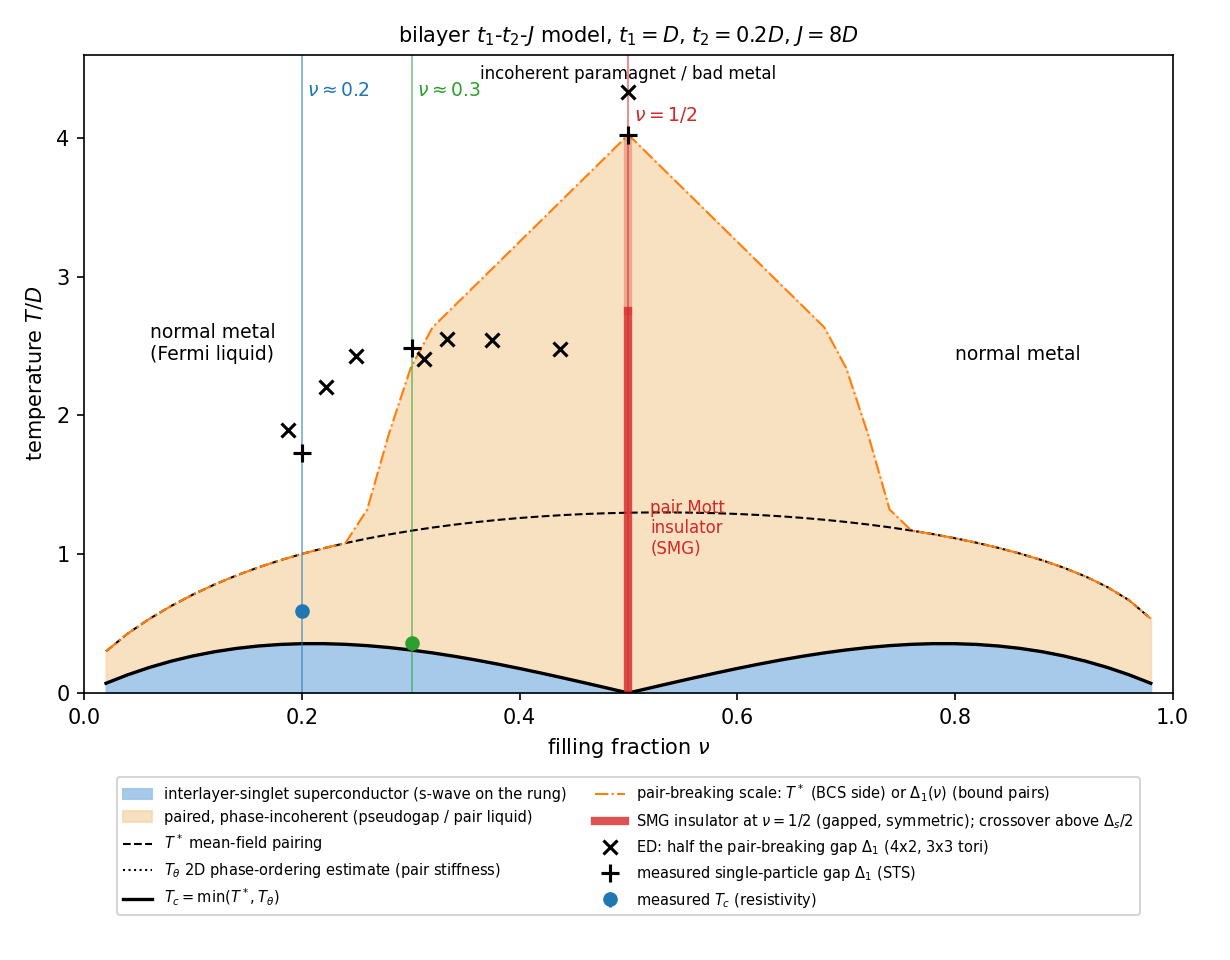
\includegraphics[width=0.9\textwidth]{phase_diagram.png}
\caption{Phase diagram of Eq.~\eqref{eq:H} at $t_1=1$, $t_2=0.2$, $J=8$. Dashed: mean-field pairing temperature $T^*(\nu)$ in the inter-layer singlet channel ($g=3J/4$). Dotted: estimate of the two-dimensional phase-ordering temperature from the pair stiffness (hard-core pair bosons with hopping interpolating between the exact two-body value $0.68$ and the strong-coupling value $0.33$; it vanishes at the pair-Mott point $\nuh$). Solid: $T_c=\min(T^*,T_\theta)$. Dash-dotted: single-particle gap, the scale below which the spin excitations are gapped (pseudogap). The red bar is the symmetric gapped insulator at $\nuh$. Circles: measured $T_c$. Crosses: half the pair-breaking gap $E_{N+1}+E_{N-1}-2E_N$ from exact diagonalization ($\nu=0.19$--$0.44$ on the $4\times2$ torus; $\nu=0.22$, $0.33$ and $\nuh$ on the $3\times3$ torus); plus signs: the measured single-particle gaps.}
\label{fig:pd}\end{figure}

Figure~\ref{fig:pd} is built from three calculations (\texttt{code/bcs.py}, \texttt{code/phase\_diagram.py}): (i) the BCS mean-field theory of Eq.~\eqref{eq:H} in the inter-layer singlet channel, $J\mathbf S_1\!\cdot\!\mathbf S_2=-\tfrac34J\,b^\dagger b+\dots$ with $b^\dagger=(c^\dagger_{1\uparrow}c^\dagger_{2\downarrow}-c^\dagger_{1\downarrow}c^\dagger_{2\uparrow})/\sqrt2$, solved with the gap and number equations on the $t_1$-$t_2$ band (this gives $\Delta=1.73$, $T^*=1.00$ at $\nu=0.2$ and $\Delta=2.12$, $T^*=1.17$ at $\nu=0.3$); (ii) the exact two-body problem (one rung pair in the empty band is bound by only $0.33$ and has effective hopping $0.68$: the dilute limit is BCS-like, not a Bose gas); (iii) the strong-coupling expansion around the singlet product state near $\nuh$ (Sec.~\ref{sec:sc}). The phase-stiffness line uses the Kosterlitz--Thouless value for hard-core bosons on the square lattice, $T_{KT}=0.685\,t_b$ at half pair filling, scaled by $4n_b(1-n_b)$ with the pair density $n_b=2\nu$.

\textbf{Phases.} (1) $\nuh$: symmetric gapped insulator at all temperatures of the window; it has no phase transition on warming, only crossovers at $T\sim\Delta_s/2\approx3$ (spin gap) and $T\sim\Delta_c/2\approx4$ (charge gap) to an incoherent paramagnet; for $|\nu-\tfrac12|$ small it extends as a thermally activated insulator. (2) $0<\nu<\tfrac12$ and $\tfrac12<\nu<1$: inter-layer singlet $s$-wave superconductor below $T_c(\nu)$, a dome that vanishes at $\nu\to0,1$ (no carriers) and at $\nuh$ (pairs form a Mott insulator). The two sides are not mirror images because $t_2$ makes the band asymmetric: the mean-field $T^*$ and the stiffness are smaller on the electron-doped side. (3) Between $T_c$ and the pair-breaking scale near $\nuh$: paired, phase-incoherent liquid with a pseudogap (the single-particle gap fills but does not close). (4) Elsewhere above $T_c$: a normal Fermi-liquid metal.

\textbf{The three crystals, low to high $T$.} $\nuh$: symmetric gapped insulator (SMG) $\to$ (crossover near $T\sim3$--$4$) incoherent paramagnetic insulator/bad metal. $\nut$: superconductor ($T<0.36$) $\to$ paired, spin-gapped, insulating-like pair liquid ($0.36<T\lesssim3$) $\to$ incoherent metal (Korringa relaxation and bare-band tunnelling DOS at $T\ge4$). $\nutw$: superconductor with sharp Bogoliubov quasiparticles ($T<0.59$) $\to$ Fermi-liquid metal.

\textbf{Where the data fall.} The measured $T_c=0.36$ at $\nu=0.30$ agrees with the phase-stiffness estimate ($0.31$) and lies far below $T^*=1.17$ and below the measured gap ($2.5$), which is the signature of the BEC-like, stiffness-limited regime. The measured $T_c=0.59$ at $\nu=0.20$ lies above the two-dimensional phase-ordering estimates ($0.25$ from the diamagnetic stiffness of the paired bilayer, $0.36$ from the hard-core pair bosons; the Kosterlitz--Thouless bound set by the full diamagnetic stiffness of the two layers is $\approx0.4$) and well below the mean-field pair-breaking temperature $T^*=1.00$, with $2\Delta/T_c=5.9$: here too the transition is set by phase coherence rather than by pair breaking, and the excess over the strictly two-dimensional estimates (a factor $1.6$) is what the Josephson coupling between the blocks of a three-dimensional crystal adds to the stiffness. The pairs are small at this density as well ($k_F\xi\approx0.7$ with $\xi=v_F/\pi\Delta$), but the Bogoliubov quasiparticles stay sharp. The mean-field gap at $\nu=0.2$ ($1.73$, with $\mu=-2.47$) coincides with the measured values, and the gap at $\nu=0.3$ ($2.12$) is $15\%$ below the measured $2.49$, as expected from a mean-field decoupling at $J=8$.

\section{Task 3: what in the theory produces each measurement}\label{sec:data}

\begin{figure}[h]\centering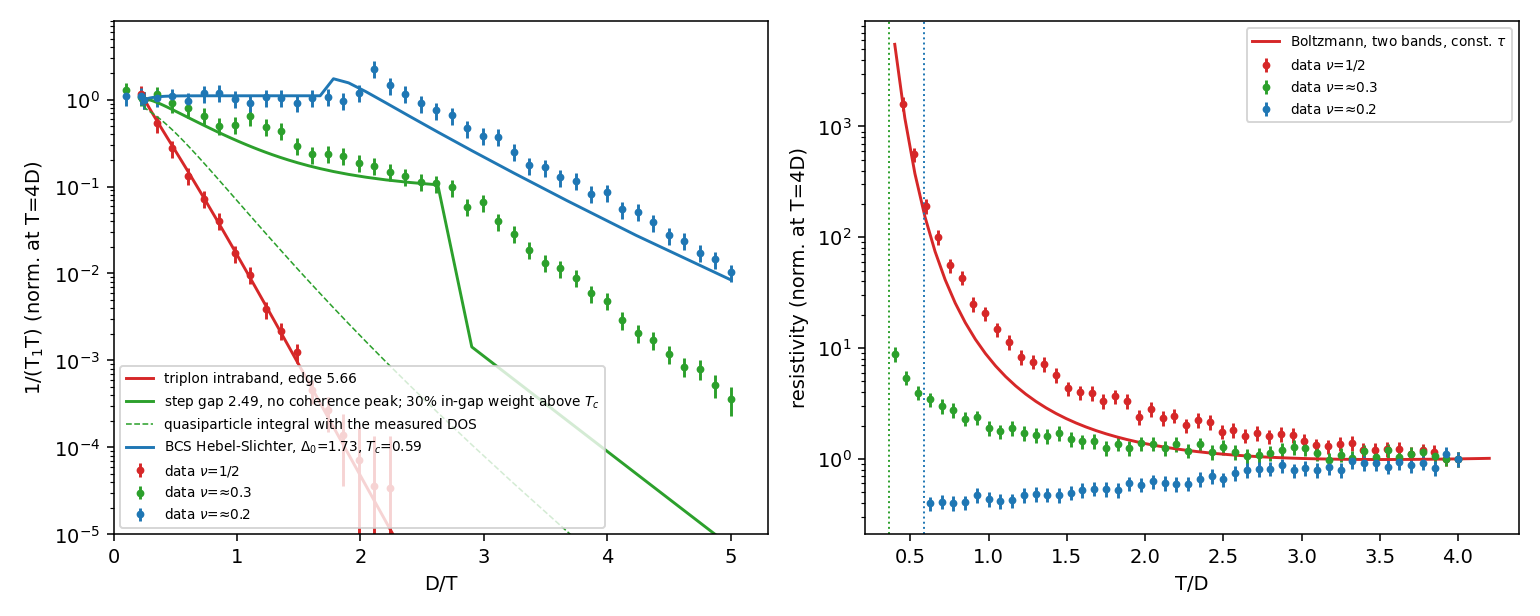
\includegraphics[width=0.98\textwidth]{nmr_resistivity_model.png}
\caption{Model curves (lines) against the data. Left: $1/(T_1T)$ from intraband triplon scattering at $\nuh$ (ED-calibrated triplon band), from a step-edged gap of $2.49$ without coherence peak, with $30\%$ in-gap weight above $T_c$ (solid) and from the quasiparticle integral with the measured DOS (dashed) at $\nut$, and from the BCS Hebel--Slichter integral at $\nutw$; all curves are normalized at $T=4$. Right: constant-$\tau$ Boltzmann resistivity of the holon and trion bands at $\nuh$; dotted lines mark the measured $T_c$ of the doped crystals.}
\label{fig:models}\end{figure}

\textbf{Diffraction.} The rung-singlet insulator and the on-rung $s$-wave superconductor are invariant under every lattice symmetry; the unit cell stays one rung and the metal sites stay equivalent, so no peak appears or splits. The competing orders of this band (antiferromagnetism or an exciton condensate at the nesting vector $(1/2,1/2)$, charge order) would double the cell, and a uniform inter-layer exciton condensate would make the two layers inequivalent; the diffraction and the single NMR line exclude them at all three fillings.

\textbf{STS (a), $\nuh$.} Hard gap $\Delta_c=\tfrac32J-4t_1=8$ between the holon band ($\omega\in[-8,-4]$) and the trion band ($[4,8]$), each the bare band with half its width (Sec.~\ref{sec:sc}); the van Hove peaks of $\varepsilon(k)/2$ sit at $-5.2$ and $+6.8$ because the van Hove point lies $2t_2$ above the centre of each side band; the particle side is heavier ($1.08$) because the residues are not equal beyond first order ($n(k)>\tfrac12$ where $\varepsilon(k)<0$, Sec.~\ref{sec:arpes}). The tunnelling DOS vanishes identically inside the gap and is the same on every site because the state is uniform.

\textbf{STS (b), $\nut$, low $T$.} The full gap ($\pm2.49$) is the pair-breaking energy of inter-layer singlet pairs in the strongly paired regime. The absence of a sharp coherence peak and the gradual rise of the DOS above the edge follow from the proximity to the pair-Mott insulator: at $\nu=0.30$ sixty percent of the rungs are singlets and the single-particle excitation is a holon propagating through them, which is damped by the pair liquid rather than a sharp Bogoliubov quasiparticle. The weight is asymmetric (peak heights $0.41$ against $0.95$, integrated weights $0.90$ against $2.03$) for the same reason as in (a): the holon-like removal states have smaller residue. The outer edges at $-5.9$ and $+6.9$ are the bottom of the holon band and the top of the trion-like band. Exact diagonalization of the model at this density gives a pair-breaking gap $E_{N+1}+E_{N-1}-2E_N=4.8$ on the $4\times2$ torus (10 electrons, $\nu=0.31$) and $5.10$ on the $3\times3$ torus (12 electrons, $\nu=0.33$), i.e.\ a single-particle gap $\Delta_1=2.4$--$2.55$, against the measured $2.49$; the lowest spin-1 excitation of the same clusters lies at $3.4$--$3.6$ ($4\times2$) and $4.1$ ($3\times3$), below the two-quasiparticle continuum $2\Delta_1$: a bound rung triplet (a remnant of the triplon of the insulator) survives in the paired state. The exact $n(k)$ of the $3\times3$ cluster at $\nu=0.33$ falls from $0.77$ at $(0,0)$ to $0.09$ at $(1/2,1/2)$ and is far broader than a Bogoliubov occupation with $\Delta=2.5$ (a BCS fit of it needs $\Delta_{\rm eff}=4.1$): the pairs are small, which is the same statement as the absence of a coherence peak.

\textbf{STS (c), $\nutw$, low $T$.} BCS density of states of the $t_1$-$t_2$ band with an isotropic gap $\Delta=1.73$ and $\mu=-2.46$: square-root coherence peaks at $\pm\Delta$, the van Hove peak displaced to $\sqrt{(4t_2-\mu)^2+\Delta^2}=3.7$, the occupied part of the band ending at $-\sqrt{(\varepsilon_{\min}-\mu)^2+\Delta^2}=-3.0$ and the empty part at $+6.0$. The fit in Fig.~\ref{fig:fits}(c) is quantitative. The fitted $\mu$ lies $0.54$ below the normal-state value of the same density ($-1.92$ for a filling of $0.20$): pairing at fixed density pulls the chemical potential down, and with these values the occupied fraction $\sum_kv_k^2$ is $0.200$ while the normal-state filling of $\mu=-2.46$ would be only $0.16$. The mean-field theory of Eq.~\eqref{eq:H} at $\nu=0.2$ gives exactly these numbers ($\Delta=1.73$, $\mu=-2.47$; Sec.~3), exact diagonalization gives $\Delta_1=1.8$--$2.0$ at $\nu=0.19$ (6 electrons on the $4\times2$ torus, periodic/antiperiodic) and $2.20$ at $\nu=0.22$ (8 electrons on the $3\times3$ torus), and the exact $n(k)$ of the $3\times3$ cluster at $\nu=0.22$ is a Bogoliubov occupation to within $0.02$ with $\mu=-2.5$ and $\Delta_{\rm eff}=2.5$: the model reproduces the gap, the shift of the chemical potential and the occupation of this crystal without any adjustment.

\textbf{STS (d), $\nut$, high $T$.} With the thermal broadening removed this is the bare single-particle DOS of Eq.~\eqref{eq:H} with $J$ ineffective: one band of width $8t_1$, lower edge $-4t_1-4t_2-\mu$, upper edge $4t_1-4t_2-\mu$, van Hove peak at $4t_2-\mu=+1.7$. The NMR of this crystal reaches its Korringa value only for $T\ge4$, so the trace was taken at $T\gtrsim4$, above the pairing (pseudogap) scale; this also explains the larger noise, since a thermal deconvolution at high $T$ amplifies it.

\textbf{NMR $1/(T_1T)$, $\nuh$.} The only low-energy spin fluctuations are thermally excited triplons scattering within their band (a two-dimensional band with a constant DOS at its bottom), which gives $1/T_1\propto T e^{-\Delta_s/T}$, i.e.\ $1/(T_1T)\propto e^{-\Delta_s/T}$ with $\Delta_s$ the triplon edge at $(1/2,1/2)$. The ED triplon band of the $3\times3$ torus ($8.47$ at $(0,0)$, $7.36$ at $(1/3,0)$, $6.33$ at $(1/3,1/3)$; $\omega_t(k)=7.03+0.70(\cos k_x+\cos k_y)+0.03\cos k_x\cos k_y$) has its edge at $(1/2,1/2)$ at $5.66$ ($5.43$ directly on the $4\times2$ torus) and a width of $2.8$; the relaxation rate computed from it (Fig.~\ref{fig:models}) has an Arrhenius slope of $5.8$ over $T\le2$, against the measured $5.5\pm0.2$. The spin gap is smaller than the charge gap ($\tfrac32J-4t_1$) because a triplon costs $J$ and gains kinetic energy only in second order, while a holon and a trion each cost $\tfrac34J$ and gain $2t_1$ each in first order. A single NMR line follows from the uniformity of the state and the absence of a static moment.

\textbf{NMR, $\nut$.} Two activated regimes and no Hebel--Slichter peak. Below $T_c=0.36$ the slope is $2.47\pm0.09$, the tunnelling half-gap $2.49$: a nuclear spin flip needs a thermally excited quasiparticle above the full gap, and there is no coherence peak because the DOS has no square-root singularity at the edge (a step-edged gap gives exactly $e^{-\Delta_1/T}$, Fig.~\ref{fig:models}; the same integral with the measured, gradually rising DOS would give an apparent slope of $3.5$). Between $T_c$ and $T\approx2$ the slope drops to $1.03\pm0.10$ although the tunnelling gap is $2.5$: above $T_c$ the pairs survive but lose phase coherence, and the phase fluctuations fill the gap from inside rather than closing it, so the relaxation is carried by the in-gap weight (the model curve of Fig.~\ref{fig:models} assumes $30\%$ in-gap weight just above $T_c$, growing to the full DOS at $T^*\approx4$, and reproduces both slopes). One feature of the data is not reproduced by any quasiparticle model: the rate is continuous through $T_c$ and is still $10\%$ of its Korringa value at $T_c=\Delta_1/7$, where relaxation across a gap of $2.49$ would give $e^{-7}\approx10^{-3}$; the magnitude of the curve below $T_c$ (a factor $\approx40$ above the quasiparticle integral) therefore has to be read for its slope only, or as a relaxation channel through the bound pairs themselves (the rung triplet of Sec.~4, STS (b)) that persists across $T_c$. The Korringa value is reached only at $T\ge4$, where the STS trace (d) is also that of the bare band: between $0.36$ and $\approx4$ this crystal is the pseudogap (pair-liquid) state, which is also why its resistance above $T_c$ rises on cooling.

\textbf{NMR, $\nutw$.} Above $T_c=0.59$ the Korringa law of a Fermi liquid. Just below $T_c$ the coherence factors of an $s$-wave BCS state give the Hebel--Slichter peak (model with a Dynes broadening of $0.05$: $1.7\times$ Korringa at $T=0.56$, against the measured $2.27\times$ at $0.47$), followed by $e^{-\Delta/T}$ with the measured slope $1.74\pm0.06$ equal to the tunnelling gap $1.73$.

\textbf{Resistivity, $\nuh$.} Transport by thermally excited holons and trions: with a constant scattering time, $\rho^{-1}\propto\sum_k v_k^2(-\partial f/\partial E_k)$ over both bands, which is activated with $\Delta_c/2=4$ corrected by the energy dependence of the velocity and the DOS (the Boltzmann curve of Fig.~\ref{fig:models} has an apparent slope $4.3$ over the window; the data give $3.72$, the difference indicating a scattering rate that grows with the carrier energy). The activation energy is half the tunnelling gap and is not the spin gap: NMR and transport measure different excitations, which is itself a signature of the singlet insulator.

\textbf{Resistivity, $\nut$.} Zero below $T_c=0.36$. Above it the carriers are bound pairs (and a few thermally broken ones): the pair liquid near the Mott point is a bad conductor whose resistance grows on cooling with a small activation ($0.90$, of order the pair hopping scale), until phase coherence sets in. \textbf{Resistivity, $\nutw$.} Zero below $T_c=0.59$, and above it the metallic, decreasing-on-cooling resistance of a Fermi liquid with a small Fermi surface (filling $0.20$, $\mu_N=-1.92$).

\section{Task 4: predicted low-temperature ARPES intensity}\label{sec:arpes}

\begin{figure}[h]\centering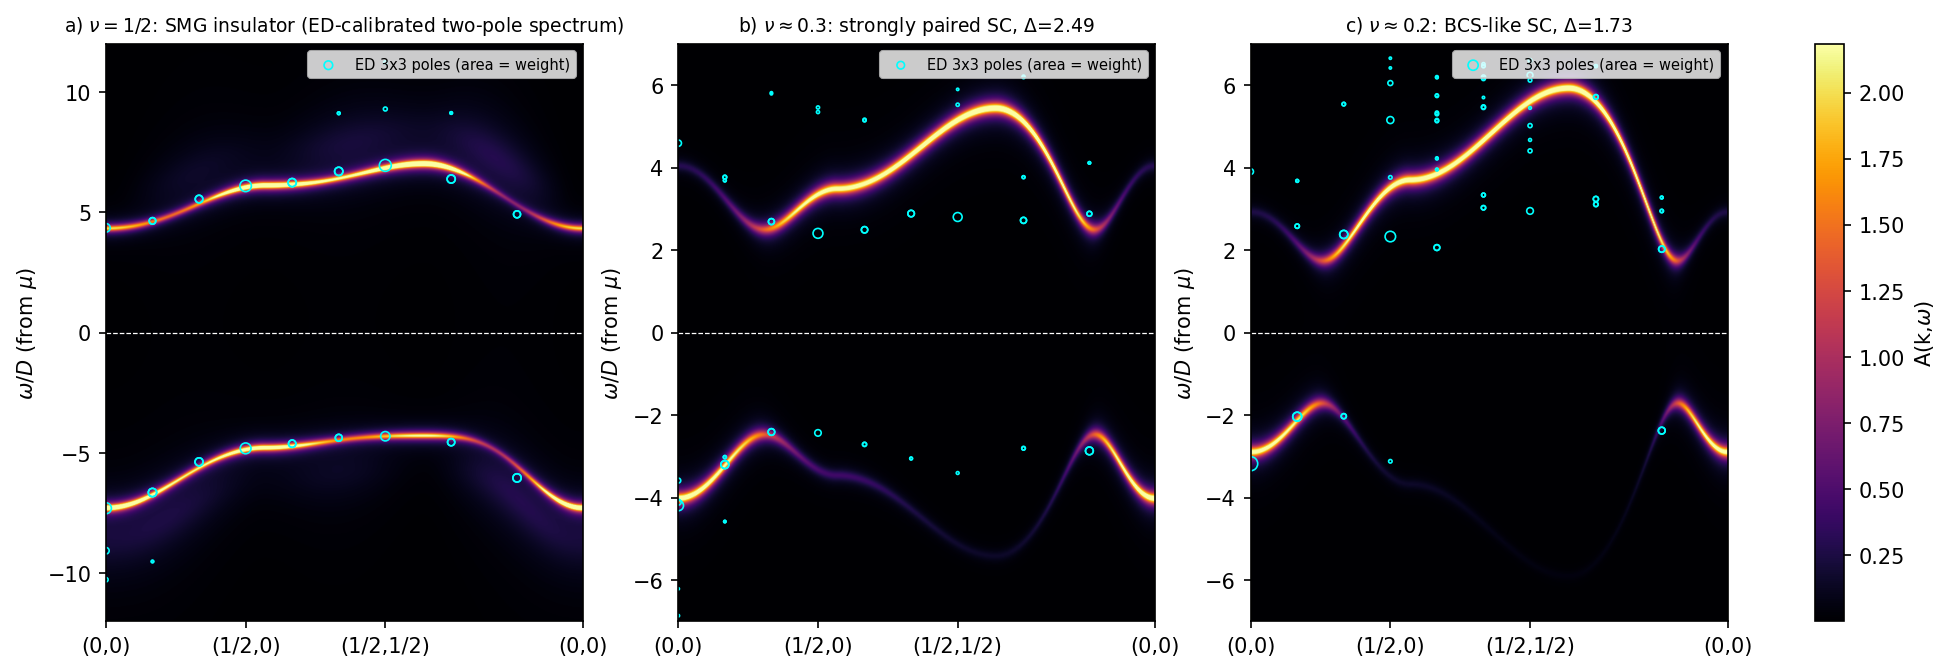
\includegraphics[width=0.99\textwidth]{arpes.png}
\caption{Predicted $I(k,\omega)/f(\omega)=A(k,\omega)$ along $(0,0)\to(1/2,0)\to(1/2,1/2)\to(0,0)$, energies from the chemical potential. (a) $\nuh$: strong-coupling two-pole spectrum calibrated on the 3$\times$3 bilayer ED (circles: exact cluster poles, area $\propto$ weight). (b) $\nut$: Bogoliubov spectrum with the measured gap. (c) $\nutw$: BCS spectrum with the fitted $\Delta$ and $\mu$.}
\label{fig:arpes}\end{figure}

\begin{figure}[h]\centering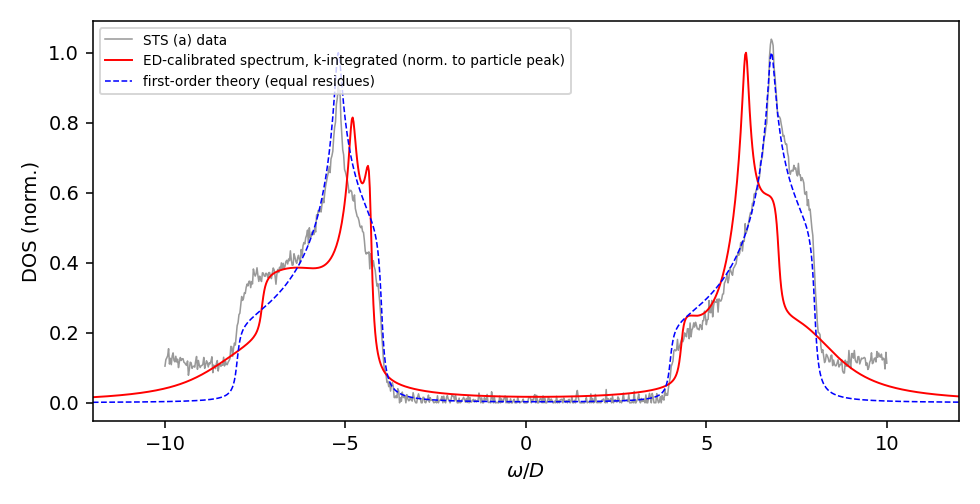
\includegraphics[width=0.8\textwidth]{sts_half_model.png}
\caption{$k$-integrated spectrum at $\nuh$: STS (a) (grey), the ED-calibrated spectrum of Fig.~\ref{fig:arpes}(a) integrated over the zone (red) and the leading-order spectrum with equal residues (blue dashed), with the same broadening.}
\label{fig:stshalf}\end{figure}

\textbf{(a) $\nuh$.} No Fermi surface and no spectral weight within $\pm4$ of $\mu$ anywhere in the zone. Two bands are seen, and both disperse \emph{in the same direction} along the path: the removal (holon) band from $-7.3$ at $(0,0)$ through $-4.9$ at $(1/2,0)$ to its top $-4.3$ at $(1/2,1/2)$, and the addition (trion) band from its bottom $+4.3$ at $(0,0)$ through $+5.8$ at $(1/2,0)$ to $+7.0$ at $(1/2,1/2)$ (ED-calibrated values; leading order: $-8\to-4.4$ and $+3.6\to+8$). The two bands are shifted copies of each other, $E_p(k)-E_h(k)=11.3$--$11.6\approx\tfrac32J$ at every $k$, and each is a copy of the bare band with reduced width: the slopes $dE/d\varepsilon$ are $0.39$ (removal) and $0.33$ (addition) in the exact spectra against $0.5$ at leading order, i.e.\ coherent widths $3.0$ and $2.7$ against $4.0$. Two parallel bands separated by $\tfrac32J$ are the fingerprint of the rung-singlet insulator; in a band insulator, a density wave or a BCS state the two bands bend away from each other (particle--hole mirror). The weights are strongly momentum dependent: the removal residue is $0.46$ at $(0,0)$, $0.45$ at $(1/2,0)$ and $0.34$ at $(1/2,1/2)$, the addition residue $0.28$, $0.51$ and $0.55$; $n(k)$ itself falls smoothly from $0.71$ at $(0,0)$ to $0.34$ at $(1/2,1/2)$ and crosses $1/2$ near the contour $\varepsilon(k)\approx0.1$, close to the bare Fermi surface ($\varepsilon=0.48$), but without a discontinuity (the fraction of the zone with $n(k)>1/2$ is $0.43$). The rest of the weight is incoherent and lies beyond the coherent bands ($0.25$ at $-9.9$ for $k=(0,0)$, $0.11$ at $+10.1$ for $(1/2,1/2)$; at generic momenta the cluster splits the weight between two poles $0.4$--$0.6$ apart, which in the thermodynamic limit is a broadened band); it is drawn with a width of $1.2$. The measured side bands of STS (a) have the full leading-order width $4.0$ (Fig.~\ref{fig:stshalf}); if the ARPES bands turn out $4$ wide rather than $3$ the leading-order spectrum is the better description, but the qualitative features (two parallel bands, no crossing, transfer of weight from the removal to the addition side across the bare Fermi surface) are the same. Thermal broadening by triplons scales as $e^{-\Delta_s/T}$ and is negligible below $T\approx1$. Energy window: $\pm12$.

\textbf{(b) $\nut$.} A Bogoliubov spectrum of the bare band with an isotropic gap $\Delta=2.49$: one band that back-bends at the minimum-gap locus, with weight $v_k^2$ below and $u_k^2$ above $\mu$. With $\mu=-1.63$ from the number equation at $\nu=0.301$ the locus is the contour $\varepsilon(k)=-1.63$, which crosses the path at $(0.27,0)$ and $(0.19,0.19)$ and encloses $0.23$ of the zone (the normal-state Fermi surface, $\varepsilon=-0.91$, crosses at $(0.31,0)$ and $(0.21,0.21)$ and encloses $0.30$; the shrinking of the locus is the fixed-density effect of strong pairing, and it is what the exact $n(k)$ at $\nu=0.33$ shows). The band has its minimum $\pm2.49$ on the locus, reaches $4.1$ at $(0,0)$ (almost pure removal weight), $3.5$ at $(1/2,0)$ and $5.5$ at $(1/2,1/2)$ (almost pure addition weight). The back-bending is smeared and the coherence peaks are weak because the pairs are small (Sec.~\ref{sec:data}); the exact poles of the $3\times3$ cluster at $\nu=0.33$ (circles) show the gap $2.5$, the removal weight concentrated at $(0,0)$ and $(1/3,0)$ and the addition weight spread over many poles between $2.5$ and $10$: a holon moving through the pair liquid is not a sharp quasiparticle. The spectrum is particle--hole asymmetric, the addition side carrying twice the removal weight (STS (b): $2.0$ against $0.9$). Window: $\pm7$.

\textbf{(c) $\nutw$.} The same Bogoliubov form with $\Delta=1.73$ and $\mu=-2.46$ (the STS fit, which coincides with the mean-field solution at fixed density $0.20$): sharp back-bending on the minimum-gap locus $\varepsilon(k)=-2.46$, which crosses the path at $(0.23,0)$ and $(0.16,0.16)$ and encloses $0.16$ of the zone, i.e.\ it lies \emph{inside} the normal-state Fermi surface of the same density ($0.20$ of the zone, crossing at $(0.26,0)$ and $(0.18,0.18)$) because pairing has pulled $\mu$ down by $0.54$; the removal band runs from $-3.0$ at $(0,0)$ up to $-1.73$ at the locus and loses its weight beyond it, the addition band from $+1.73$ at the locus to $+3.7$ at $(1/2,0)$ (the van Hove flattening) and $+6.0$ at $(1/2,1/2)$. Sharp quasiparticles throughout (coherence peaks in STS, Hebel--Slichter peak in NMR). The exact poles at $\nu=0.22$ (circles) follow the removal branch ($-3.2$ at $(0,0)$, $-2.0$ at $(1/3,0)$) with a gap of $2.2$, and again spread the addition weight over many poles. Window: $\pm7$.

\textbf{Comparison.} (i) Gaps: $8.6$ (ED; $8.0$ measured) at $\nuh$ with no minimum-gap locus; $2.49$ at $\nut$ with a smeared locus enclosing $0.23$ (normal-state Fermi surface: $0.30$); $1.73$ at $\nutw$ with a sharp locus enclosing $0.16$ (normal-state Fermi surface: $0.20$). In both superconductors the locus lies inside the normal-state Fermi surface, by the amount pairing lowers $\mu$ at fixed density. (ii) Band topology: at $\nuh$ the removal and addition bands are parallel, both rising from $(0,0)$ to $(1/2,1/2)$ and separated by $\tfrac32J$; in the superconductors they are mirror images about $\mu$ that bend away from each other at the locus. (iii) Dispersion: $3$--$4$ wide at $\nuh$ (half the bare width or less), the full bare dispersion ($8$) in the superconductors. (iv) Weights: at $\nuh$ a continuous transfer of weight from the removal to the addition band across the zone ($n(k)$ from $0.71$ to $0.34$); at $\nutw$ a $v_k^2$ step at the locus smeared over $\Delta/v_F\approx0.2\pi$; $\nut$ in between, with the broad $n(k)$ of small pairs. (v) Incoherent weight: large and $k$-selective at $\nuh$ (satellites $2.5$--$3.5$ beyond the bands), spread over the whole addition side at $\nut$, small at $\nutw$. The $\nut$ spectrum interpolates between the other two: its addition side occupies the energy range of the trion band of the insulator while its removal side still shows the back-bending of a superconductor.

\section{Task 5: Green's function zeros and the Luttinger count}

\begin{figure}[h]\centering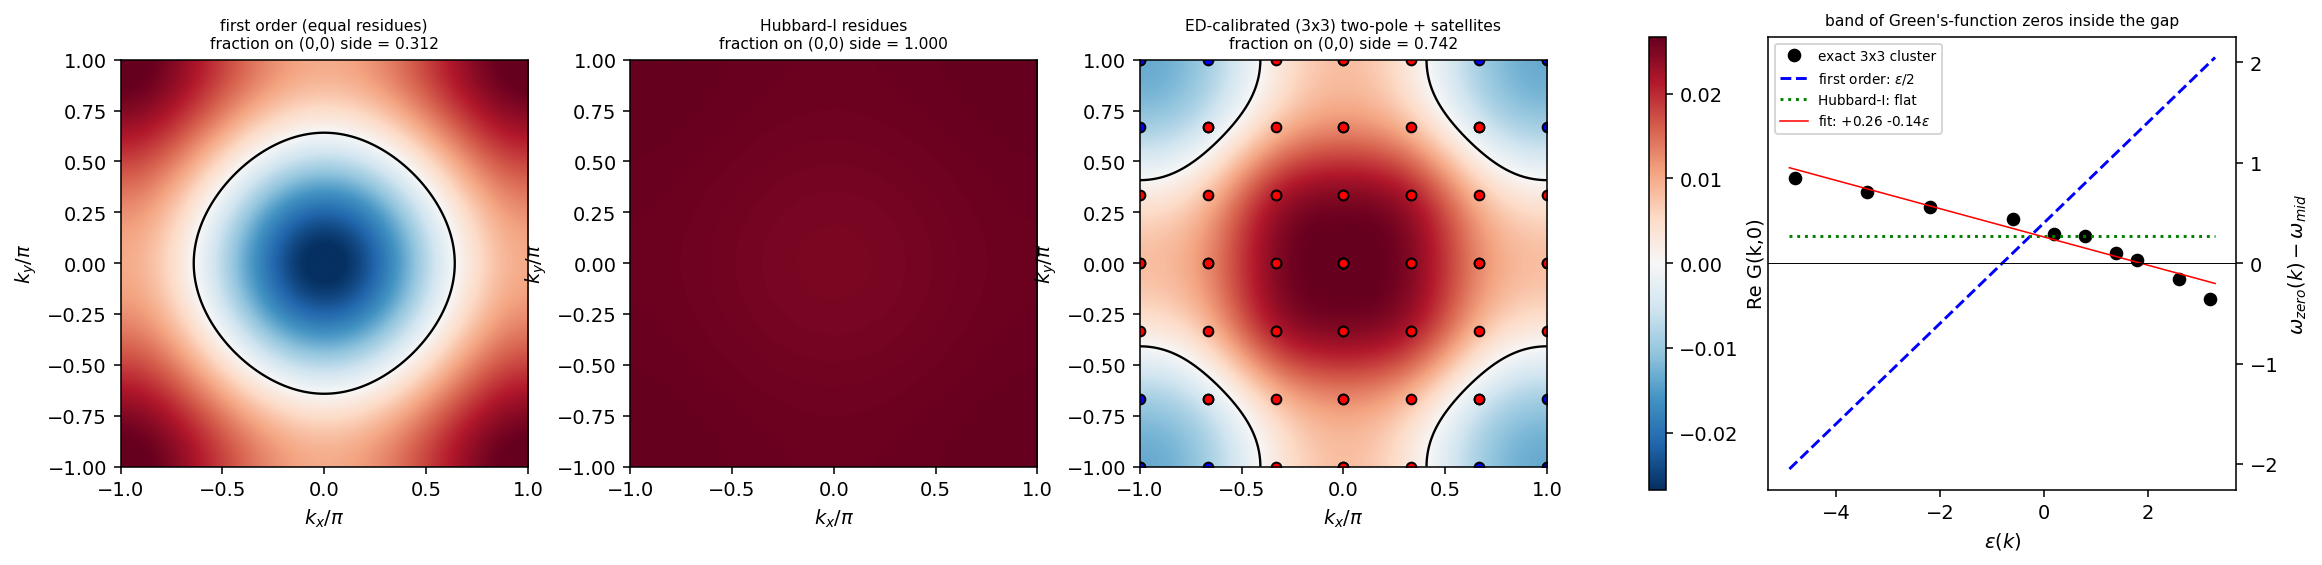
\includegraphics[width=0.99\textwidth]{luttinger.png}
\caption{$\mathrm{Re}\,G(k,\omega=0)$ at $\nuh$ (from $\mathrm{Re}\,G(k,0)=-\int A(k,\omega')\,d\omega'/\omega'$), with $\omega$ measured from the gap midpoint; black: the zero surface. Left: first-order theory; middle: Hubbard-I residues; right: ED-calibrated spectrum, with the sign of the exact cluster Green's function at the 3$\times$3 grid points (red $>0$, blue $<0$).}
\label{fig:lutt}\end{figure}

\textbf{Procedure and result.} With $A(k,\omega)$ of Fig.~\ref{fig:arpes}(a) ($\int A\,d\omega=1$, removal part $=n(k)$) and $\omega$ measured from the gap midpoint, $\mathrm{Re}\,G(k,0)=-\mathcal P\!\int A(k,\omega')\,d\omega'/\omega'$, which for a pole representation is $-\sum_jZ_j(k)/E_j(k)$. $G(k,0)$ is real and has no poles, so its sign changes only on a surface of zeros. For the ED-calibrated spectrum of Fig.~\ref{fig:arpes}(a) the fraction of the zone on the $(0,0)$ side of that surface is $0.74$ (Fig.~\ref{fig:lutt}, third panel; the zero surface is the contour $\varepsilon(k)\approx1.5$, closed around $(1/2,1/2)$). The exact cluster values at the ten momenta of the $6\times6$ grid have the same signs ($G>0$ for $\varepsilon(k)\le1.8$, $G<0$ for $\varepsilon(k)\ge2.6$) and interpolate to a zero contour $\varepsilon(k)=1.9$, i.e.\ a fraction $0.81$. We quote $0.74$--$0.81$, against $\nu=0.50$.

\textbf{Why it is not $\nu$.} For a metal the Luttinger theorem equates the volume inside the Fermi surface ($G^{-1}=0$) with the density; its extension to insulators counts the volume inside the surface of zeros, $\nu=\mathrm{vol}\{\mathrm{Re}\,G(k,0)>0\}$, and rests on the existence of the Luttinger--Ward functional, i.e.\ on the self-energy being reachable perturbatively from the free band. The gap of the rung-singlet insulator is not of that kind, and the calculations show how the count fails. (i) Leading order: $G=\tfrac12/(\omega-E_p)+\tfrac12/(\omega-E_h)$ vanishes on $\omega=\varepsilon(k)/2$ (plus the midpoint offset), a \emph{band of zeros} with half the bare dispersion; at $\omega=0$ its zero surface is $\varepsilon(k)=\tfrac12(\varepsilon_{\max}+\varepsilon_{\min})=-4t_2$ and encloses $0.31$. With particle--hole symmetry ($t_2=0$) it would be $\varepsilon=0$ and enclose exactly $1/2$: the theorem holds at this order only by symmetry, and $t_2$ breaks it. (ii) Hubbard-I residues give $G=\omega/(\omega^2-\varepsilon\omega-36)$, whose zero band is flat, $\omega=0$ for all $k$: the zero surface is then the whole zone or nothing, and the fraction is undefined (a midpoint offset of $-0.27$ turns this into the ``$1.000$'' of the second panel). (ii$'$) A residue asymmetry of the phenomenological form used for zeros in symmetric-mass-generation insulators, $Z_{p,h}=\tfrac12\pm\varepsilon(k)/4J$ on the leading-order poles (Lu, Zeng and You, arXiv:2307.12223), gives a zero band $\omega_{\rm zero}-\omega_{\rm mid}=(\tfrac12-\tfrac{3J}{8J})\varepsilon=0.125\,\varepsilon$, i.e.\ a zero contour $\varepsilon(k)=-3.2$ closed around $(0,0)$ that encloses only $0.10$ of the zone, with $\mathrm{Re}\,G<0$ inside. The general rule for two poles $E_{p,h}=\pm\tfrac34J+s\,\varepsilon$ with residues $\tfrac12\mp\beta\varepsilon$ is $\omega_{\rm zero}-\omega_{\rm mid}=(s-\tfrac32J\beta)\,\varepsilon$ (up to the midpoint offset): the slope of the zero band, and with it the side of the zone on which $\mathrm{Re}\,G>0$ and the enclosed fraction, is the difference of two comparable numbers, the band slope and the residue slope. Leading order has $\beta=0$; the phenomenological form has $\tfrac32J\beta=0.375<s=0.5$ (zero band rising with $\varepsilon$, small fraction around $(0,0)$ with $G<0$); the exact cluster has $\tfrac32J\beta=0.57>s=0.33$--$0.39$ (zero band falling with $\varepsilon$, large fraction with $G>0$). (iii) Exact cluster (fourth panel): the zero band exists, is nearly flat and disperses in the \emph{opposite} direction, $\omega_{\rm zero}(k)-\omega_{\rm mid}=0.26-0.14\,\varepsilon(k)$ (total dispersion $1.2$ inside a gap of $8.6$), because the incoherent weight sits on the removal side at $(0,0)$ and on the addition side at $(1/2,1/2)$; it crosses the midpoint at $\varepsilon(k)\approx1.9$. Because the zero band is so flat, the enclosed fraction is hypersensitive to the reference energy: a shift of $\pm0.3$ ($3\%$ of the gap, less than the uncertainty of a gap midpoint in a real spectrum) moves it between $0.46$ and $0.91$, and keeping only the main poles moves it to $0.10$; with the residues of (ii$'$) it would be $0.10$ with the opposite sign at $(0,0)$. The zero surface of this insulator is therefore not a conserved quantity like a Fermi surface: its location depends on $t_2/t_1$ (through the midpoint offset) and on the residues, not on a theorem, and its departure from $\nu$ is not a small correction but the statement that the Luttinger--Ward construction does not apply to a symmetric gap generated by $J$. The count that does hold is the sum rule $2\sum_kn(k)/N_k=1$ electron per site, with $n(k)$ passing through $1/2$ close to the bare Fermi surface but continuously (Sec.~\ref{sec:arpes}).

\section{Methods, approximations and system sizes}

\textbf{Fits (\texttt{code/fit\_data.py}).} Least-squares fits of the full STS traces with the model densities of states described in Sec.~1 (bare band; two half-width side bands; BCS), each convolved with a Gaussian of fitted width and with the $V^2$ background outside the gap; weighted Arrhenius fits of $1/(T_1T)$ and $\ln\rho$.

\textbf{Strong-coupling expansion (\texttt{code/strong\_coupling.py}).} Exact two-rung problem (256 states) and degenerate second-order perturbation theory in $t$ around the singlet product state: first-order holon/trion hopping $t/2$ (exact), second-order triplon hopping $4t^2/J$ and bond energies, pair-boson hopping $8t^2/3J$ and interaction $4t^2/J$. Second order is only marginal at $J=8$ (the virtual holon--trion pairs cost $3J/2=12$ while the two bands they occupy are $8$ wide), which is why the gaps and bands were taken from exact diagonalization.

\textbf{Mean field (\texttt{code/bcs.py}).} BCS decoupling of $J\mathbf S_{i1}\!\cdot\!\mathbf S_{i2}$ in the inter-layer singlet channel ($g=3J/4$), gap and number equations on a $400\times400$ $k$ grid at $T=0$ and at finite $T$ (pairing temperature $T^*$); $T=0$ diamagnetic stiffness. Exact two-body (one pair) bound state and dispersion by the Lippmann--Schwinger equation.

\textbf{Exact diagonalization (\texttt{code/ed\_gpu.py}).} Lanczos diagonalization of Eq.~\eqref{eq:H} on periodic bilayer tori, with the many-body vector stored as a matrix $\Psi[u,d]$ over up- and down-spin configurations: hopping acts as $H_\uparrow\Psi+\Psi H_\downarrow^{T}$, the Ising part of $J$ as an element-wise mask and the spin flips as $\sum_r A_r\Psi B_r^{T}$ with sparse one-hop matrices, all as sparse--dense products on the GPU (PyTorch, double precision). Sectors used: $4\times2$ bilayer (16 sites; $1.66\times10^8$ states at half filling, $0.13$\,s per matrix--vector product, 10\,GB) and $3\times3$ bilayer (18 sites; $2.36\times10^9$ states at half filling, $2.2$\,s per product with row-chunked temporaries, 48\,GB on one H200). Single-particle and triplon spectral functions from Lanczos continued fractions ($70$--$160$ steps) started from $c^{(\dagger)}_{k\ell\sigma}|0\rangle$ and $\sum_r e^{ikr}(S^+_{r1}-S^+_{r2})|0\rangle$; periodic/antiperiodic boundary conditions in each direction give $k$ grids shifted by half a step, i.e.\ a $6\times6$ grid on the $3\times3$ torus (for the spin-flip operator $S^+_q$, which carries the difference of two single-particle momenta, the allowed $q$ stay on the unshifted grid, so only the periodic run gives momentum-resolved triplon poles; the twisted runs give the lowest $S=1$ state, $6.27$--$6.33$ at $(1/3,1/3)$, as a measure of the twist dependence). The zeros of $G$ were found from the full pole sums of the cluster, $\mathrm{Re}\,G(k,\omega)=\sum_jZ_j/(\omega-E_j)$, solved for $\omega$ inside the gap at each momentum (\texttt{code/luttinger.py}). Validation: the GPU energies agree with an independent sparse-matrix construction on the $2\times2$ bilayer to $10^{-13}$ in five sectors and boundary conditions; spectral sum rules $\langle cc^\dagger\rangle+\langle c^\dagger c\rangle=1$ and $\sum_k n(k)=N_\uparrow$ hold to $10^{-8}$; at $J=0$ the poles reproduce $\varepsilon(k)$ exactly and at $J=100$ the first-order bands $\pm\tfrac34J+\varepsilon(k)/2$ to $0.01$. Hardware choice: one product takes $4.2$\,s on 32 CPU cores against $0.037$\,s on the GPU for the $1.9\times10^7$-state sector ($110\times$), so every production run used the two GPUs; the full set of runs took about five GPU-hours ($4\times2$: $1.2$\,h; $3\times3$ gaps: $0.7$\,h; $3\times3$ twisted grid: $2.5$\,h; $J$ derivatives and tests: $0.5$\,h). Limitations: on the $4\times2$ torus the bonds along the short direction are double-counted, which reproduces $\varepsilon(k)$ at the allowed momenta but over-weights second-order processes along that direction and makes $(1/2,0)$ and $(0,1/2)$ inequivalent at $J=8$ (they are degenerate again at $J=100$); the isotropic $3\times3$ torus is free of this but has a coarse grid, hence the twisted boundary conditions. Finite-size effects in the gapped state are small because the correlation length is below one lattice spacing.

\textbf{Transport and relaxation (\texttt{code/transport\_nmr.py}).} Constant-$\tau$ Boltzmann conductivity of the two half-filled bands; $1/(T_1T)\propto T^{-1}\int d\epsilon\,\rho_t(\epsilon)^2 n_B(\epsilon)[1+n_B(\epsilon)]$ with the ED-calibrated triplon DOS $\rho_t$; BCS Hebel--Slichter integral with a Dynes broadening $\Gamma=0.05$ and $\Delta(T)=\Delta_0\tanh(1.74\sqrt{T_c/T-1})$; for $\nut$ the same integral without coherence factors, with a step-edged gap equal to the tunnelling half-gap and a phenomenological in-gap weight ($30\%$ just above $T_c$, growing linearly to the full DOS at $T^*=4$), and, for comparison, with the measured symmetrized tunnelling DOS.

\end{document}
